\section{Boundary activity and the packing contradiction}
\label{sec:boundary}

We now use the spatial measure constructed above to rule out the assumed
sequence of extremal batches. The essential finite observation is that,
when the directions of the cutting lines vary little, every participating
vertex either lies in one of three narrow strips or is accounted for by
a marked token crossing the boundary of a fixed region. We first prove
this observation without taking limits.

\begin{lemma}[Three strips]
\label{lem:three-strips}
Let $P$ be a finite subset of $\mathbb R^2$, let $B$ be a bounded open set,
and let $D\geq1$ satisfy $|x|\leq D$ for $x\in B$. Suppose that
$M_0,\ldots,M_m\subset P$ have the same cardinality and are given by
strictly separating cuts
\[
 M_i=\{x\in P:\nu_i\cdot x<c_i\},
 \qquad |\nu_i|=1,
 \qquad |\nu_i-\nu_0|\leq\theta.
\]
For each $i\geq1$, choose a bijection from $M_{i-1}\setminus M_i$ to
$M_i\setminus M_{i-1}$. Let $C_B$ count the resulting transfers having
exactly one endpoint in $B$, and let
\[
 A=\bigcup_{i=1}^m(M_{i-1}\mathbin\triangle M_i)
\]
be the set of distinct participating vertices. Set
\[
 \rho=D\theta,\qquad c_- =\min_{0\leq i\leq m}c_i,
 \qquad c_+=\max_{0\leq i\leq m}c_i,
\]
and, for $q\in\{c_0,c_-,c_+\}$, define the closed strip
\[
 S_q=\{x\in\mathbb R^2:|\nu_0\cdot x-q|\leq3\rho\}.
\]
Then
\[
 \#\bigl((A\cap B)\setminus(S_{c_0}\cup S_{c_-}\cup S_{c_+})\bigr)
 \leq2C_B,
\]
and consequently
\begin{equation}
 \#(A\cap B)
 \leq 2C_B+
 \sum_{q\in\{c_0,c_-,c_+\}}\#(P\cap B\cap S_q).
 \label{eq:finite-three-strips}
\end{equation}
Repeated thresholds may be counted repeatedly in the sum.
\end{lemma}

\begin{proof}
Write $t(x)=\nu_0\cdot x$ and
$e_i(x)=(\nu_i-\nu_0)\cdot x$. For $x\in B$ we have
$|e_i(x)|\leq\rho$, and $e_0(x)=0$. Put
$S=S_{c_0}\cup S_{c_-}\cup S_{c_+}$.
Figure~\ref{fig:three-strip-projection} shows the two ranges in which
participants in $B$ outside $S$ can occur. We compare their membership with
the states attaining the minimum and maximum thresholds.

\begin{figure}[htbp]
\centering
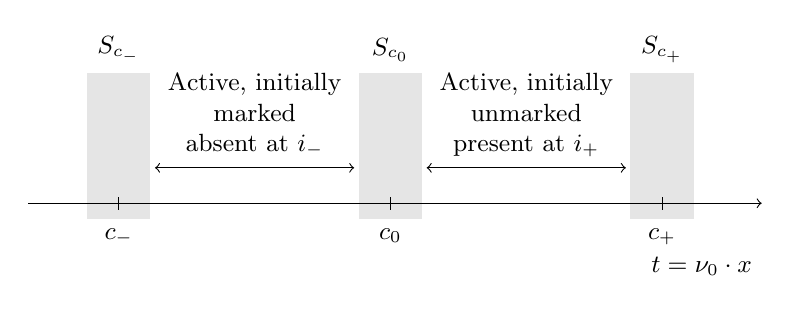
\begin{tikzpicture}[x=1.15cm,y=1cm,font=\small]
  \fill[gray!20] (.65,-.2) rectangle (1.35,1.65);
  \fill[gray!20] (3.65,-.2) rectangle (4.35,1.65);
  \fill[gray!20] (6.65,-.2) rectangle (7.35,1.65);
  \draw[->] (0,0)--(8.1,0);
  \draw (1,-.08)--(1,.08);
  \draw (4,-.08)--(4,.08);
  \draw (7,-.08)--(7,.08);
  \node[below] at (1,-.2) {$c_-$};
  \node[below] at (4,-.2) {$c_0$};
  \node[below] at (7,-.2) {$c_+$};
  \node[anchor=east] at (8.1,-.8) {$t=\nu_0\cdot x$};
  \node at (1,1.95) {$S_{c_-}$};
  \node at (4,1.95) {$S_{c_0}$};
  \node at (7,1.95) {$S_{c_+}$};
  \draw[<->] (1.4,.45)--(3.6,.45);
  \draw[<->] (4.4,.45)--(6.6,.45);
  \node[align=center] at (2.5,1.12)
    {Active, initially\\marked\\absent at $i_-$};
  \node[align=center] at (5.5,1.12)
    {Active, initially\\unmarked\\present at $i_+$};
\end{tikzpicture}
\caption{Projection onto $t=\nu_0\cdot x$. The shaded bands have
half-width $3\rho$; their separation is schematic, and in general they
may overlap. An initially marked participant in $B$ outside the bands is lost
by a state $i_-$ attaining $c_-$; this endpoint comparison has no gains
inside $B$.
The symmetric statement holds for initially unmarked participants and
a state $i_+$ attaining $c_+$. Token conservation bounds these two
numbers by exits and entries, respectively. This is an aggregate count;
it does not assign each participant's own token to a boundary crossing.}
\label{fig:three-strip-projection}
\end{figure}

Consider first an $x\in(A\cap B)\setminus S$ that is initially marked.
Avoidance of $S_{c_0}$ gives $t(x)<c_0-3\rho$. Since $x$ participates,
it is unmarked at some boundary state, and hence
$t(x)+e_i(x)>c_i\geq c_-$ at some $i$. Therefore
$t(x)>c_- -\rho$. Avoidance of $S_{c_-}$ improves this to
$t(x)>c_-+3\rho$. At an index $i_-$ attaining the minimum threshold,
\[
 \nu_{i_-}\cdot x\geq t(x)-\rho>c_-;
\]
thus $x$ is lost between states $0$ and $i_-$. The existence of even one
such $x$ also forces $c_0-c_->6\rho$. Consequently every initially
unmarked $y\in P\cap B$ is still unmarked at state $i_-$, because
\[
 \nu_{i_-}\cdot y\geq t(y)-\rho>c_0-\rho>c_-.
\]
There are therefore no gains anywhere inside $B$ in this comparison,
including among vertices lying in the strips.

To count the losses, place one distinct token on each point of $M_0$.
At every step retain the tokens on unchanged marked vertices and move
the others along the chosen matching. There is exactly one token on
every marked vertex at each state. It follows that
\[
 \#(M_0\cap B)-\#(M_{i_-}\cap B)
 =\text{token exits from }B-\text{token entries into }B
\]
over that prefix of steps. Since all differences between these two states inside $B$ are losses,
their number equals this difference and is at most $C_B$. This bounds
the initially marked participants outside the strips; if there are
none, the bound holds without imposing a threshold gap.

Now let $x\in(A\cap B)\setminus S$ be initially unmarked. It satisfies
$t(x)>c_0+3\rho$ and is marked at some later state, so
$t(x)<c_++\rho$. Avoidance of $S_{c_+}$ implies
$t(x)<c_+-3\rho$. At an index $i_+$ attaining $c_+$,
\[
 \nu_{i_+}\cdot x\leq t(x)+\rho<c_+,
\]
so $x$ is gained by that state. If this class is nonempty, then
$c_+-c_0>6\rho$. Every initially marked $y\in P\cap B$ consequently
remains marked at state $i_+$, since
\[
 \nu_{i_+}\cdot y\leq t(y)+\rho<c_0+\rho<c_+.
\]
All differences between these two states inside $B$ are gains, and token
conservation bounds their number by $C_B$. The two classes together
contain at most $2C_B$ vertices, proving
\eqref{eq:finite-three-strips}.

The argument includes $\theta=0$, when the strips are lines. It also
includes vertices that change membership several times and return to
their initial status: participation requires only that some boundary
state differs from the initial one.
\end{proof}

We apply this lemma only to states separating consecutive batches.
Thus its set $A$ is exactly the set of endpoints participating in the
batch exchange graph. A membership change within a batch followed by
a return before its end does not by itself contribute a vertex to $A$
or to the measure $\mu_J$; that vertex may still participate at another
batch boundary.

For the rest of this section, suppress the tildes on the enhanced
measures from Section~\ref{sec:spatial}, and write $\widetilde Z$ for
their compact label space, which includes compactified Euclidean position. The
condition $z\in G$ always refers to the old rank label, pulled back to
$\widetilde Z$. Thus expressions such as $\mu_J(G)$ refer to the
enhanced measures restricted by that condition.

Recall the particular inputs furnished by the preceding construction.
There is a dyadic window $K_0$, a measurable label set $G$, and limiting
measures with
\begin{equation}
 \begin{gathered}
 \lambda_{K_0}(G)>0,\qquad \mu_J\leq\mu,\qquad
 \lambda_J(\widetilde Z)=|J|,\\
 \lambda_J(F)^3\leq C s_J^3\mu_J(F).
 \end{gathered}
 \label{eq:boundary-measure-input}
\end{equation}
for every Borel set $F\subset\widetilde Z$ and every dyadic $J\subset K_0$.
Here $s_J$ is the limiting fraction of distinct participating batch
endpoints. At every dyadic resolution $\delta$,
\begin{equation}
 \#\{J\subset K_0:|J|=\delta,\ s_J>u\}
 \leq C u^{-4/3}.
 \label{eq:boundary-packing-input}
\end{equation}
The spatial projection $\beta$ of $\mu|_G$ is boundedly supported and
satisfies
\begin{equation}
 \beta(B(x,r))\leq C_G r^d,
 \qquad 0<r<1,
 \qquad d=\frac{32}{17}>\frac74.
 \label{eq:boundary-disk-input}
\end{equation}
These masses are unchanged because the enhancement preserved all the
original measure projections.

The directions throughout $K_0$ lie between the directions at its two
fixed bracketing times. The common linear normalization sends those
two projective directions to distinct fixed directions. Passing to a
subsequence selects one of the two projective arcs between them and
one of its two oriented lifts. Hence all forward transfer vectors lie
in a fixed closed cone $\mathcal C$ of aperture less than $\pi$.
We may enlarge this cone slightly and discard finitely many indices. Each intermediate
forward transfer vector is a positive linear combination of the two
bracketing forward vectors; this identifies the relevant cone after
normalization, including its orientation.

Choose linearly independent covectors $\ell_1,\ell_2$ in the interior
of its dual cone. Thus $\ell_j(v)>0$ for every nonzero
$v\in\mathcal C$. Choose a bounded open parallelogram
\[
 B=\{x:a_1<\ell_1(x)<b_1,\ a_2<\ell_2(x)<b_2\}
\]
whose interior contains the support of $\beta$, and fix
$D\geq\max(1,\sup_{x\in B}|x|)$.

For every batch choose one perfect matching between its $a$ lost and
$a$ gained marked vertices, making this choice once throughout $K_0$.
Follow the resulting system of at most $N$ marked tokens. Each side
functional is monotone along every token trajectory, so each token
crosses each of the four side levels of $B$ at most once. Therefore
there are at most $4N$ matching transfers with one endpoint inside $B$
and one outside during the entire window $K_0$.

Let $C_n(J)$ be the number of these transfers during $J$ in
configuration $n$. Let $\theta_n(J)$ be the angular width of the span
of its boundary-state directions in the normalized plane. These
directions rotate monotonically, and the spans of disjoint windows
have disjoint interiors. Thus, for every dyadic partition of $K_0$,
\[
 \sum_J \frac{C_n(J)}{N_n}\leq4,
 \qquad \sum_J\theta_n(J)\leq\pi.
\]
A diagonal subsequence on the countable family of windows gives
limits $b_J$ and $\theta_J$ with
\begin{equation}
 \sum_J b_J\leq4,\qquad \sum_J\theta_J\leq\pi.
 \label{eq:boundary-budgets}
\end{equation}
These are limits at a fixed time resolution; no assertion of uniform
convergence over resolutions is needed.

\begin{lemma}[Limiting boundary activity]
\label{lem:limiting-boundary-activity}
For each dyadic $J\subset K_0$,
\begin{equation}
 \mu_J(G)\leq2b_J+C_G\theta_J^{d-1}.
 \label{eq:limiting-boundary-activity}
\end{equation}
\end{lemma}

\begin{proof}
Apply Lemma~\ref{lem:three-strips} to the finite boundary states of
$J$. Continuously orient their unit normals so that the marked sets
are given by $\nu_i\cdot x<c_i$. Their angular span is
$\theta_n(J)$, and consequently $|\nu_i-\nu_0|\leq\theta_n(J)$.

Pass further to a subsequence so that the initial normal and the
initial, minimum and maximum thresholds converge, allowing infinite
threshold limits. This can be done simultaneously for the countably
many windows. A finite threshold limit gives a limiting closed strip
of half-width $3D\theta_J$. A threshold tending to either infinity
gives strips that eventually miss every bounded set. Let $\mathcal S_J$ be
the union of the nonescaping limiting strips.

Let $\alpha_n$ be the spatial projection of the participating-vertex
measure in $J$, normalized by $N_n$, and let $\alpha$ be its weak
limit. Any continuous function $f$ with $0\leq f\leq1$ and compact
support in $B\setminus\mathcal S_J$ eventually avoids all three moving strips.
Lemma~\ref{lem:three-strips} therefore gives
\[
 \int f\,d\alpha_n\leq 2C_n(J)/N_n.
\]
Passing to the limit and exhausting the open set by such tests yields
$\alpha(B\setminus\mathcal S_J)\leq2b_J$. Since the positions carrying
$\mu|_G$ lie inside $B$, and $\mu_J\leq\mu$, it follows that
\[
 \mu_J(G)\leq2b_J+\beta(\mathcal S_J).
\]
This argument restricts to $G$ only after weak convergence; no
convergence of finite restrictions to $G$ has been assumed.

To bound the remaining term, cover the intersection of a strip of
half-width $r$ with the bounded support of $\beta$ by $O_G(r^{-1})$
disks of radius $O(r)$. Equation~\eqref{eq:boundary-disk-input} gives
\[
 \beta(\text{strip of half-width }r)\leq C_G r^{d-1}
 \qquad(0<r<1).
\]
For larger widths the same estimate follows from the total mass bound
after increasing $C_G$. A line has zero $\beta$-mass by continuity
from above, since $d>1$. Applying this bound to the at most three
limiting strips proves the result, including $\theta_J=0$.
\end{proof}

It remains to combine this activity bound with the endpoint estimate.
Fix $M\geq1$ and subdivide $K_0$ into dyadic windows of length
$\delta$. By \eqref{eq:boundary-packing-input}, the number with
$s_J>M\delta^{3/4}$ is at most
$C M^{-4/3}\delta^{-1}$. Each has total $\lambda_J$-mass $\delta$,
so these windows contribute at most $C M^{-4/3}$ to
$\lambda_{K_0}(G)$.

For the other windows, \eqref{eq:boundary-measure-input} gives
\[
 \sum_{s_J\leq M\delta^{3/4}}\lambda_J(G)
 \leq C M\delta^{3/4}\sum_J\mu_J(G)^{1/3}.
\]
There are at most $\delta^{-1}$ windows. Set
$\alpha=d-1=15/17\in(0,1)$. H\"older's inequality,
Lemma~\ref{lem:limiting-boundary-activity}, and
\eqref{eq:boundary-budgets} imply
\[
 \sum_J\mu_J(G)^{1/3}
 \leq \delta^{-2/3}\Bigl(\sum_J\mu_J(G)\Bigr)^{1/3}
 \leq C_G\delta^{-2/3}
       \Bigl(1+\sum_J\theta_J^\alpha\Bigr)^{1/3}.
\]
Concavity and the angular budget give
\[
 \sum_J\theta_J^\alpha
 \leq \delta^{\alpha-1}\Bigl(\sum_J\theta_J\Bigr)^\alpha
 \leq C\delta^{\alpha-1}.
\]
Consequently
\begin{align*}
 \lambda_{K_0}(G)
 &\leq C M^{-4/3}
      +C_G M\delta^{-1/4}(\delta+\delta^{d-1})^{1/3}\\
 &\leq C M^{-4/3}
      +C_G M\bigl(\delta^{1/12}+\delta^{3/68}\bigr),
\end{align*}
where
\[
 \frac{d-1}{3}-\frac14
 =\frac{15}{51}-\frac14=\frac{3}{68}>0.
\]
First let $\delta\downarrow0$ with $M$ fixed, and then let
$M\to\infty$. This contradicts $\lambda_{K_0}(G)>0$ and excludes
the proposed sequence of extremal batches. Together with the finite
reductions, it establishes the uniform little-$o$ activity-packing
estimate. The numerical exponent $3/68$ concerns only this limiting
contradiction; the power saving in the final finite theorem is chosen
separately.
